\section*{One Year Horizon}

\begingroup
\setlength{\columnsep}{16pt}

\begin{wrapfigure}{r}{3in}
\vspace{-0.4in}

  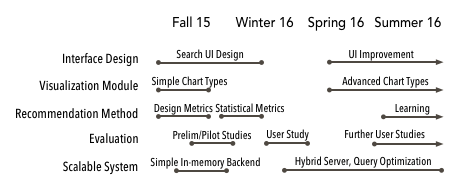
\includegraphics[width=3in]{gantt-chart.png}
  \vspace{-0.3in}
  \caption{Timeline during the 2015-2016 Academic Year}

\label{fig:plan}
\vspace{-0.1in}
\end{wrapfigure}


This research is a multi-year project.  We expect to deliver a working system for general datasets that fit in memory in the first year.

Figure 3 shows our project timeline during the 2015-2016 Academic Year.
in the beginning, we will focus on developing and evaluating user interfaces and recommendation algorithms.
The initial system will support commonly used chart types including histogram, bar chart, line chart, scatter plot and map.
We will perform a lab study comparing our recommender system with existing tools such as Tableau.
We will measure the rate of events such as participants’ observations, generalizations and questions during the analysis sessions \cite{liu:latency}.

\endgroup

During the first half of the year, we will also start the implementation of the backend server.  In the latter half of the year, we will focus on scaling the system to support higher volume of data and advanced visualization types. We will also improve our user interface and recommender algorithm based on user study results, and run further user studies.


